% =============================================================================
%  Cyclistic — professional report (Google Data Analytics capstone), English edition
%  Build: see README.md (XeLaTeX, three passes, or python -I scripts/build_latex_report.py)
% =============================================================================
\documentclass[11pt, a4paper, oneside, headings=normal, numbers=noenddot]{scrartcl}
\usepackage{cyclistic-eisvogel}
\graphicspath{{../../visualizations/}}

% --- Metadata (edit in one place) -------------------------------------------------
\newcommand{\ReportAuthor}{LUMU BAMANA MANASSE}
\newcommand{\ReportShortTitle}{Cyclistic — case study}
\newcommand{\ReportTitle}{Cyclistic: annual members\\and casual riders}
\newcommand{\ReportSubtitle}{Two ways of using a bike-share service:\\an analysis of 6,012,458 rides and three recommendations}
\newcommand{\ReportContext}{Google Data Analytics Professional Certificate\par\smallskip
  Case Study 1: \textit{How does a bike-share navigate speedy success?}}
\newcommand{\ReportMeta}{%
  \begin{tabularx}{\linewidth}{@{}l@{\hspace{0.8em}}Y@{}}
  \textbf{Author:} & \ReportAuthor \\[0.35em]
  \textbf{Report date:} & 11 October 2026 \\[0.35em]
  \textbf{Data period:} & rides started from 1 October 2025 to 30 September 2026 \\[0.35em]
  \textbf{Source:} & Divvy public trip data (Chicago), used under the Divvy Data License Agreement \\[0.35em]
   & \textcolor{accent}{\url{https://divvy-tripdata.s3.amazonaws.com/index.html}}
  \end{tabularx}}
\hypersetup{pdftitle={Cyclistic: annual members and casual riders}, pdfauthor={\ReportAuthor},
  pdfsubject={Google Data Analytics capstone — Cyclistic case study}, pdflang={en-US}}

\begin{document}
\MakeTitlePage

% --- Contents ---------------------------------------------------------------------
\pagenumbering{roman}
\setcounter{tocdepth}{2}
\begingroup
\addtokomafont{sectionentry}{\color{accent}}
\tableofcontents
\endgroup
\clearpage
\pagenumbering{arabic}

\addsec{Reading guide and key terms}

This report covers the six phases of the project (\emph{Ask, Prepare, Process, Analyze, Share, Act}).
Each key statement carries a status label: \Mes{} fact measured in the data;
\Int{} interpretation of the measurements; \Hyp{} marketing hypothesis to be validated through experimentation.
The figures in the tables are generated automatically from the analysis files (Appendix~\ref{sec:repro}).

\begin{table}[H]
\caption{Terms and labels used in this report}
\label{tab:terms}
\small
\begin{tabularx}{\linewidth}{L{3.3cm} Y}
\toprule
\thead{Term} & \thead{Meaning} \\
\midrule
Ride & Unit of analysis: one bike rental, from unlocking to docking. The data set contains no rider identifier: we count \textbf{rides}, never people. \\
Member / casual & The \texttt{member\_casual} field of the source: annual membership (\emph{member}) or single-ride and full-day passes (\emph{casual}). \\
Median & The value that splits rides into two equal halves; the main duration indicator, because a few very long rides pull the mean upwards. \\
Round trip & A ride that ends at the station where it started; computed only for rides with both a start and an end station. \\
Peak hours & Weekday departures between 7 and 9 a.m. and between 4 and 7 p.m. (Chicago local time). \\
v3.2 & Version of the data-cleaning rules applied (documented in \file{docs/plan\_nettoyage\_v3.2.md}). \\
SENS-1, SENS-2 & Sensitivity analyses: with or without positive rides shorter than 60~s; with or without 31~March and 1~April 2026. \\
A/B test & Controlled comparison of two versions of a message shown to randomly assigned groups. \\
\bottomrule
\end{tabularx}
\end{table}

\clearpage
\section{Executive summary}
\label{sec:summary}

\textbf{Question.} How do annual members and casual riders use Cyclistic bikes differently?
The business goal, set by the marketing director, is to convert more casual riders into annual members.

\textbf{Data.} 6,012,458 rides started between 1~October 2025 and 30~September 2026, after documented and verified data cleaning (72 quality checks, raw data left unchanged).

\begin{center}
\begin{minipage}[t]{0.235\linewidth}\keyfig{member}{64.8\%}{of rides are taken by annual members}\end{minipage}\hfill
\begin{minipage}[t]{0.235\linewidth}\keyfig{casual}{11.2~vs~8.7}{minutes of median ride duration, casual riders vs members}\end{minipage}\hfill
\begin{minipage}[t]{0.235\linewidth}\keyfig{casual}{37\% vs 23\%}{of rides take place at the weekend, casual riders vs members}\end{minipage}\hfill
\begin{minipage}[t]{0.235\linewidth}\keyfig{casual}{×14~vs~×4.7}{ratio between the busiest and the quietest month}\end{minipage}
\end{center}

\textbf{What the data show} \Mes
\begin{itemize}
  \item \textcolor{casual}{\textbf{Casual riders}} take longer rides (median 11.2 vs 8.7~min), ride more at weekends, in the afternoon and in summer, and more often make round trips (7.4\% vs 2.2\%).
  \item \textcolor{member}{\textbf{Members}} take short, regular rides, concentrated on weekdays, with a morning peak (7--9 a.m.) twice as pronounced as among casual riders; their activity holds up in winter.
  \item A bridge exists: 62.8\% of casual rides take place on weekdays and 23.1\% start on weekdays during peak hours.
  \item The differences hold in sensitivity analyses (rides shorter than 60~s added back; 31~March and 1~April removed).
\end{itemize}

\textbf{Three recommendations, to be tested before any roll-out} \Hyp
\begin{enumerate}
  \item \textbf{Prioritize converting casual riders whose usage resembles that of members} (weekday peak-hour rides), with targeted messages evaluated through A/B testing.
  \item \textbf{Launch a leisure-oriented spring--summer campaign}, from April to June, ahead of the summer peak, evaluated against control areas.
  \item \textbf{Personalize digital communication based on ride duration and e-bike use}, after first checking the pricing structure.
\end{enumerate}

\begin{keybox}[Limitations to keep in mind]
The data describe rides, without a rider identifier, prices, pass types or weather: they show \emph{how} the bikes are used, not \emph{why}, nor how many people are behind the rides. The recommendations are hypotheses grounded in measured findings; their effectiveness remains to be demonstrated.
\end{keybox}

\section{Business context and problem}
\label{sec:context}

Cyclistic is a fictional bike-share company in Chicago whose data are those of the Divvy network: according to the case study, a fleet of 5,824 geotracked bicycles locked into a network of 692 stations, including assistive options (reclining bikes, hand tricycles, cargo bikes).
It offers single-ride passes, full-day passes and annual memberships.
According to the case study's finance analysts, \textbf{annual members are much more profitable} than casual riders.

Lily Moreno, the director of marketing, believes that future growth depends on maximizing the number of annual members and that there is an opportunity to convert casual riders, who are already aware of the service.
Three questions guide the future marketing program; this report addresses the first one.

\begin{keybox}[Assigned task]
\textbf{Question 1:} How do annual members and casual riders use Cyclistic bikes differently?\par
\smallskip
\textcolor{muted}{Questions 2 and 3, addressed by other analyses: Why would casual riders buy annual memberships? How can digital media influence them to become members?}
\end{keybox}

\textbf{Stakeholders.} Lily Moreno (project sponsor), the marketing analytics team, and the executive team, described as notoriously detail-oriented, which must approve the recommended program.

\textbf{Deliverables required by the case study.} Statement of the business task (Section~\ref{sec:context}); description of the data sources (Section~\ref{sec:data}); documentation of data cleaning (Section~\ref{sec:cleaning}); summary of the analysis (Section~\ref{sec:analysis}); visualizations and key findings (Section~\ref{sec:visuals}); three recommendations (Section~\ref{sec:recos}).

\section{Data and scope}
\label{sec:data}

\begin{table}[H]
\caption{Data source and scope}
\label{tab:scope}
\small
\begin{tabularx}{\linewidth}{L{3.6cm} Y}
\toprule
\thead{Item} & \thead{Description} \\
\midrule
Source & Divvy public trip data, Chicago (``Cyclistic'' is a fictional name), via the link provided by the case study. \\
License & Made available by Motivate International Inc. according to the case study; used under the Divvy Data License Agreement (Appendix~\ref{sec:refs}). \\
Files & 12 monthly archives, \file{202510} to \file{202609-divvy-tripdata.zip}; SHA-256 checksums recorded. \\
Period & Rides started from 1~October 2025, 12:00 a.m., to 30~September 2026, 11:59 p.m. (local time), i.e. the 12 most recent complete months. \\
Volume & 6,171,785 raw rows; 6,012,458 rides after cleaning. \\
Variables & Ride identifier, bike type (classic or electric), start and end timestamps, stations (name, identifier), coordinates, rider type. \\
Privacy & No personal data: rides cannot be linked to a person, a payment method or a place of residence (in line with the case study instructions). \\
\bottomrule
\end{tabularx}
\end{table}

\textbf{Reliability (ROCCC framework).}
\begin{itemize}
  \item \textbf{Reliable, Original:} first-party data from the operator, published monthly.
  \item \textbf{Comprehensive:} all rentals in the period, but without a rider identifier, prices, pass types or weather.
  \item \textbf{Current:} recent period (the 12 most recent complete months at the time of the analysis).
  \item \textbf{Cited:} source and license identified.
\end{itemize}

\textbf{Source characteristics detected during the audits} \Mes
\begin{itemize}
  \item The January 2026 CSV file is named \file{202501-divvy-tripdata.csv} inside the \file{202601} archive; its content does correspond to January 2026.
  \item 35 rides from 30~April to 1~May 2026 appear identically in both the April and the May files.
  \item No ride crosses the boundary from 31~March to 1~April 2026, whereas the other month boundaries have between 12 and 173: a possible gap, estimated by analogy at between 28 and 102 rides (an estimate, not a measurement).
  \item Rides started on 30~September 2026 and ended in October have not yet been published.
\end{itemize}

\section{Methodology: from question to action}
\label{sec:method}

The project follows the six phases of the Google Data Analytics process. Each phase produced a verifiable deliverable.

\begin{table}[H]
\caption{The six phases of the project and their deliverables}
\label{tab:phases}
\small
\begin{tabularx}{\linewidth}{L{2.1cm} Y L{4.6cm}}
\toprule
\thead{Phase} & \thead{Work performed} & \thead{Deliverable} \\
\midrule
\textbf{Ask} & Business task, stakeholders, question 1; scope limited to rides. & Statement of the business task (Section~\ref{sec:context}). \\
\textbf{Prepare} & Download of the 12 files, SHA-256 checksums, consistency audit (rows, columns, dates, identifiers). & Data collection audit. \\
\textbf{Process} & Raw import into PostgreSQL, cleaning plan v3.2 reviewed several times, cleaning in a single transaction, 72 quality checks. & Cleaning plan (\file{docs/}); \file{clean.trips} table; QA results (\file{results/quality/}). \\
\textbf{Analyze} & Read-only SQL aggregations, consistency checks on totals, sensitivity analyses. & 12 CSV tables (\file{results/analysis/}). \\
\textbf{Share} & Matplotlib visualizations, presentation and this report. & 11 charts; PowerPoint presentation (not included in this repository). \\
\textbf{Act} & Three recommendations with indicators and an evaluation method. & Sections~\ref{sec:recos} and~\ref{sec:measurement}. \\
\bottomrule
\end{tabularx}
\end{table}

\textbf{Tools.} PostgreSQL~18 (raw storage, cleaning, aggregations); Python with pandas and Matplotlib (checks, charts); PowerPoint (presentation); XeLaTeX (this report).

\textbf{Working principles.}
\begin{itemize}
  \item \textbf{Raw data left intact:} the raw table is never modified; its exhaustive fingerprint is checked before and after each processing step.
  \item \textbf{Traceability:} every kept or excluded ride is linked to its source row; every exclusion has a single reason.
  \item \textbf{Read-only analysis:} the aggregations write nothing to the database; the results are time-stamped CSV files with run logs.
  \item \textbf{Robust indicators:} the median is the main duration indicator; percentages are computed on each group's rides.
\end{itemize}

\section{Data cleaning, quality assurance and methodological limitations}
\label{sec:cleaning}

\subsection{Cleaning rules (version v3.2)}

Cleaning was executed in \textbf{a single PostgreSQL transaction}: had a blocking check failed, nothing would have been written.
Four exclusion rules are applied in a fixed order; each excluded row receives a single reason, and no row meets two criteria \Mes.

\begin{table}[H]
\caption{Row reconciliation: from raw data to analyzed rides}
\label{tab:cascade}
\small
% Generated by scripts/generate_latex_tables.py - do not edit by hand
\begin{tabularx}{\linewidth}{Y r r}
\toprule
\thead{Step (order of application)} & \thead{Rows excluded} & \thead{Rows remaining} \\
\midrule
Raw data (12 CSV files) &  & 6,171,785 \\
Duplicate \texttt{ride\_id} (copy in the May file) & 35 & 6,171,750 \\
Start outside the period (September 2025) & 71 & 6,171,679 \\
Negative duration (clock change) & 29 & 6,171,650 \\
Positive duration shorter than 60~s & 159,192 & 6,012,458 \\
\midrule
\textbf{Total} & \textbf{159,327} & \textbf{6,012,458} \\
\bottomrule
\end{tabularx}

\par\smallskip{\footnotesize\color{muted}Source: \file{config/attendus\_v3.2.json}, counts verified at execution time (\file{audit.transform\_log}).}
\end{table}

\begin{itemize}
  \item \textbf{60-second threshold:} Divvy's documentation states that rides shorter than 60~seconds are removed from its data (false starts, re-docking); they remained in the files, \textbf{exclusively for e-bikes}. Excluding them is a provisional choice, backed by a sensitivity analysis.
  \item \textbf{Kept, not removed globally:} rides without a station (e-bikes parked outside a station), without end coordinates or longer than 24~hours; they are left out only of the analyses that require this information.
  \item \textbf{Minimal normalization:} only leading and trailing spaces were removed from station names and identifiers; no stations were merged and no values were imputed.
  \item \textbf{Daylight saving time changes:} raw durations are kept; a correction of $-3{,}600$~s, in a separate column, applies to the 40 rides spanning the skipped hour of 8~March 2026 (four criteria checked ride by ride); no automatic correction when clocks go back in the fall.
\end{itemize}

\subsection{Quality checks}

\begin{table}[H]
\caption{Results of the 72 post-cleaning quality checks}
\label{tab:qa}
\small
\begin{tabularx}{\linewidth}{L{3.4cm} r Y}
\toprule
\thead{Status} & \thead{Count} & \thead{Comment} \\
\midrule
OK & 62 & Reconciliation raw = kept + excluded, every row matched to its source, raw data unchanged, timestamps, uniqueness, station normalization. \\
Informational & 8 & Station check lists (identifiers with several names, spatial spread) and descriptive counts. \\
Known anomaly & 1 & No March ride ending in April (a characteristic of the source, Section~\ref{sec:data}). \\
Explained failure & 1 & Maximum duration of 93,597.011~s against a reference value rounded to 93,597~s: an error in the expected value, with no effect on the data (no rule caps durations). \\
\bottomrule
\end{tabularx}
\end{table}

\subsection{Methodological limitations}
\begin{itemize}
  \item \textbf{Rides, not people:} no customer count and no individual ride frequency.
  \item \textbf{A single year:} seasonality and underlying trend cannot be separated.
  \item \textbf{Station coverage:} 20.0\% of rides have no start station and 20.8\% no end station, mostly e-bike rides; station-level analyses are deferred.
  \item \textbf{Robustness:} the differences between groups persist when rides shorter than 60~s are added back (median with / without these rides: 646.2 / 669.9~s for casual riders, 510.6 / 521.4~s for members) and when 31~March and 1~April are removed (overall median 568.0~s instead of 567.4~s).
\end{itemize}

\section{Comparative analysis of members and casual riders}
\label{sec:analysis}

Unless stated otherwise, all percentages in this section are computed on each group's rides (3,897,958 member rides, 2,114,500 casual rides). In ``A vs B'' comparisons, A refers to casual riders and B to members.

\subsection{Volume and duration}

\begin{table}[!htb]
\caption{Summary by rider type}
\label{tab:riders}
\small
% Generated by scripts/generate_latex_tables.py - do not edit by hand
\begin{tabularx}{\linewidth}{Y r r r}
\toprule
\thead{Indicator} & \thead{\textcolor{member}{Members}} & \thead{\textcolor{casual}{Casual riders}} & \thead{All} \\
\midrule
Rides & 3,897,958 & 2,114,500 & 6,012,458 \\
Share of rides & 64.8\% & 35.2\% & 100\% \\
Median duration (min) & 8.69 & 11.17 & 9.46 \\
Mean duration (min) & 12.60 & 21.11 & 15.59 \\
1st quartile / 3rd quartile (min) & 5.19 / 14.63 & 6.49 / 20.04 & 5.58 / 16.33 \\
90th percentile (min) & 23.42 & 36.05 & 27.29 \\
Rides of at least 20 min & 14.1\% & 25.1\% & 18.0\% \\
Rides of at least 30 min & 5.4\% & 13.5\% & 8.3\% \\
Rides longer than 24 hours & 1,108 & 4,196 & 5,304 \\
\bottomrule
\end{tabularx}

\par\smallskip{\footnotesize\color{muted}Source: \file{results/analysis/a01\_usagers.csv}, \file{a02\_durees\_tranches.csv}. Durations in minutes, computed from the raw timestamps.}
\end{table}

\Mes{} Nearly two rides out of three are taken by members. Casual rides are longer across the whole distribution: a median 29\% higher, a 90th percentile 54\% higher, and 13.5\% of rides lasting at least 30~min vs 5.4\%. The gap depends strongly on the season: in January, the medians are almost identical (7.13 vs 7.17~min); in June, they are 12.35 vs 9.47~min.

\subsection{Day of the week}

\begin{table}[!htb]
\caption{Distribution of rides and median duration by day of departure}
\label{tab:days}
\small
% Generated by scripts/generate_latex_tables.py - do not edit by hand
\begin{tabularx}{\linewidth}{Y r r r r}
\toprule
 & \multicolumn{2}{c}{\thead{Share of the group's rides}} & \multicolumn{2}{c}{\thead{Median duration (min)}} \\
\cmidrule(lr){2-3}\cmidrule(lr){4-5}
\thead{Day of departure} & \thead{Members} & \thead{Casual} & \thead{Members} & \thead{Casual} \\
\midrule
Monday & 14.0\% & 11.5\% & 8.41 & 10.83 \\
Tuesday & 16.1\% & 11.4\% & 8.50 & 9.89 \\
Wednesday & 16.2\% & 11.7\% & 8.49 & 9.68 \\
Thursday & 15.8\% & 12.5\% & 8.51 & 9.93 \\
Friday & 14.7\% & 15.7\% & 8.57 & 11.00 \\
Saturday & 12.8\% & 21.2\% & 9.55 & 13.06 \\
Sunday & 10.5\% & 16.0\% & 9.23 & 12.82 \\
\midrule
\textbf{Weekend (Sat.\,+\,Sun.)} & \textbf{23.3\%} & \textbf{37.2\%} & & \\
\bottomrule
\end{tabularx}

\par\smallskip{\footnotesize\color{muted}Source: \file{a03\_jour.csv}. A uniform distribution would put 28.6\% of rides at the weekend.}
\end{table}

\Mes{} The weekend accounts for 37.2\% of casual rides vs 23.3\% of member rides; Saturday is the busiest day for casual riders (21.2\%). Members ride mostly from Tuesday to Thursday. The gap in median duration is largest on Saturday (13.06 vs 9.55~min).

\subsection{Month and seasonality}

\begin{table}[!htb]
\caption{Rides and median duration by month of departure}
\label{tab:months}
\small
% Generated by scripts/generate_latex_tables.py - do not edit by hand
\begin{tabularx}{\linewidth}{L{1.9cm} R R R R R}
\toprule
\thead{Month of departure} & \thead{Member rides} & \thead{Casual rides} & \thead{Casual share} & \thead{Median, members (min)} & \thead{Median, casual (min)} \\
\midrule
Oct. 2025 & 414,231 & 214,849 & 34.2\% & 8.57 & 10.74 \\
Nov. 2025 & 252,033 & 94,930 & 27.4\% & 7.92 & 8.97 \\
Dec. 2025 & 109,411 & 27,173 & 19.9\% & 7.49 & 7.69 \\
Jan. 2026 & 109,974 & 23,962 & 17.9\% & 7.17 & 7.13 \\
Feb. 2026 & 157,270 & 40,162 & 20.3\% & 7.43 & 8.21 \\
Mar. 2026 & 223,698 & 85,031 & 27.5\% & 7.87 & 9.88 \\
Apr. 2026 & 308,523 & 127,309 & 29.2\% & 8.20 & 10.05 \\
May 2026 & 399,616 & 236,362 & 37.2\% & 8.87 & 11.83 \\
June 2026 & 444,235 & 297,844 & 40.1\% & 9.47 & 12.35 \\
July 2026 & 500,577 & 346,209 & 40.9\% & 9.36 & 11.98 \\
Aug. 2026 & 511,153 & 336,005 & 39.7\% & 9.33 & 11.76 \\
Sept. 2026 & 467,237 & 284,664 & 37.9\% & 8.90 & 11.08 \\
\midrule
\textbf{Total} & \textbf{3,897,958} & \textbf{2,114,500} & \textbf{35.2\%} & & \\
\bottomrule
\end{tabularx}

\par\smallskip{\footnotesize\color{muted}Source: \file{a04\_mois.csv}. March 2026: possible gap for rides crossing midnight on the 31st (Section~\ref{sec:data}).}
\end{table}

\Mes{} Both groups follow the same calendar, with very different amplitudes: ×14.4 between January and July for casual riders, ×4.7 between December and August for members. From May to September, casual riders take 71.0\% of their annual rides (59.6\% for members); their share of all rides ranges from 17.9\% in January to 40.9\% in July.

\subsection{Hour of departure}

\begin{table}[!htb]
\caption{Hourly indicators}
\label{tab:hours}
\small
% Generated by scripts/generate_latex_tables.py - do not edit by hand
\begin{tabularx}{\linewidth}{Y r r}
\toprule
\thead{Hourly indicator (local time of departure)} & \thead{Members} & \thead{Casual} \\
\midrule
Departures 7--9 a.m., \% of weekday rides & 15.1\% & 7.6\% \\
Departures 5--6 p.m., \% of weekday rides & 11.9\% & 10.8\% \\
Departures 10 a.m.--4 p.m., \% of weekday rides & 26.3\% & 30.7\% \\
Departures 10 a.m.--4 p.m., \% of weekend rides & 44.6\% & 45.0\% \\
Weekday peak hours (7--9 a.m. and 4--7 p.m.), \% of all the group's rides & 35.3\% & 23.1\% \\
\bottomrule
\end{tabularx}

\par\smallskip{\footnotesize\color{muted}Source: \file{a05\_heure.csv}. Local time of departure; ``7--9 a.m.'' covers departures from 7:00 to 8:59 a.m.}
\end{table}

\Mes{} On weekdays, the morning peak is twice as pronounced among members (15.1\% vs 7.6\%), while both groups peak at 5 p.m. At weekends, their hourly profiles are almost identical. \Int{} The members' double peak is consistent with commuting; part of the casual weekday rides follows the same rhythm.

\subsection{Bike type and interactions}

\begin{table}[!htb]
\caption{Bike type and type of day}
\label{tab:bikes}
\small
% Generated by scripts/generate_latex_tables.py - do not edit by hand
\begin{tabularx}{\linewidth}{Y r r r r}
\toprule
 & \multicolumn{2}{c}{\thead{Share of the group's rides}} & \multicolumn{2}{c}{\thead{Median duration (min)}} \\
\cmidrule(lr){2-3}\cmidrule(lr){4-5}
\thead{Bike, type of day} & \thead{Members} & \thead{Casual} & \thead{Members} & \thead{Casual} \\
\midrule
Classic, weekday & 24.2\% & 15.3\% & 8.92 & 14.32 \\
Classic, weekend & 7.5\% & 10.7\% & 10.09 & 17.79 \\
Electric, weekday & 52.5\% & 47.5\% & 8.33 & 9.39 \\
Electric, weekend & 15.8\% & 26.5\% & 9.13 & 11.55 \\
\midrule
\textbf{E-bike (total)} & \textbf{68.3\%} & \textbf{74.1\%} & & \\
\bottomrule
\end{tabularx}

\par\smallskip{\footnotesize\color{muted}Source: \file{a06\_velo.csv}, \file{a07\_interactions.csv}. The excluded rides shorter than 60~s were all e-bike rides.}
\end{table}

\Mes{} E-bikes account for the majority of rides in both groups. The duration gap is largest for classic bikes at weekends (17.79 vs 10.09~min) and smallest for e-bikes on weekdays (9.39 vs 8.33~min), the most frequent combination in both groups.

\subsection{Round trips}

\begin{table}[!htb]
\caption{Rides ending at their start station}
\label{tab:roundtrips}
\small
% Generated by scripts/generate_latex_tables.py - do not edit by hand
\begin{tabularx}{\linewidth}{Y R R R R}
\toprule
\thead{Group} & \thead{Rides with both stations} & \thead{Round trips} & \thead{Share of round trips} & \thead{Median round trip (min)} \\
\midrule
Members & 2,652,984 (68\%) & 58,539 & 2.2\% & 14.38 \\
Casual riders & 1,396,510 (66\%) & 103,487 & 7.4\% & 16.70 \\
\bottomrule
\end{tabularx}

\par\smallskip{\footnotesize\color{muted}Source: \file{a08\_boucles.csv}. Computed only for rides with both stations; the share of rides covered is shown in parentheses.}
\end{table}

\Mes{} Round trips are 3.4 times more frequent among casual riders. \Int{} This points to leisure use, to be confirmed by a station-level analysis.

\section{Annotated visualizations}
\label{sec:visuals}

The charts are produced by \file{scripts/figures\_analyse.py} from the CSV tables, without database access. Colors are consistent throughout: \textcolor{member}{\textbf{blue}} for members, \textcolor{casual}{\textbf{orange}} for casual riders. Each caption states the question asked, then the finding.

\begin{figure}[H]
\centering
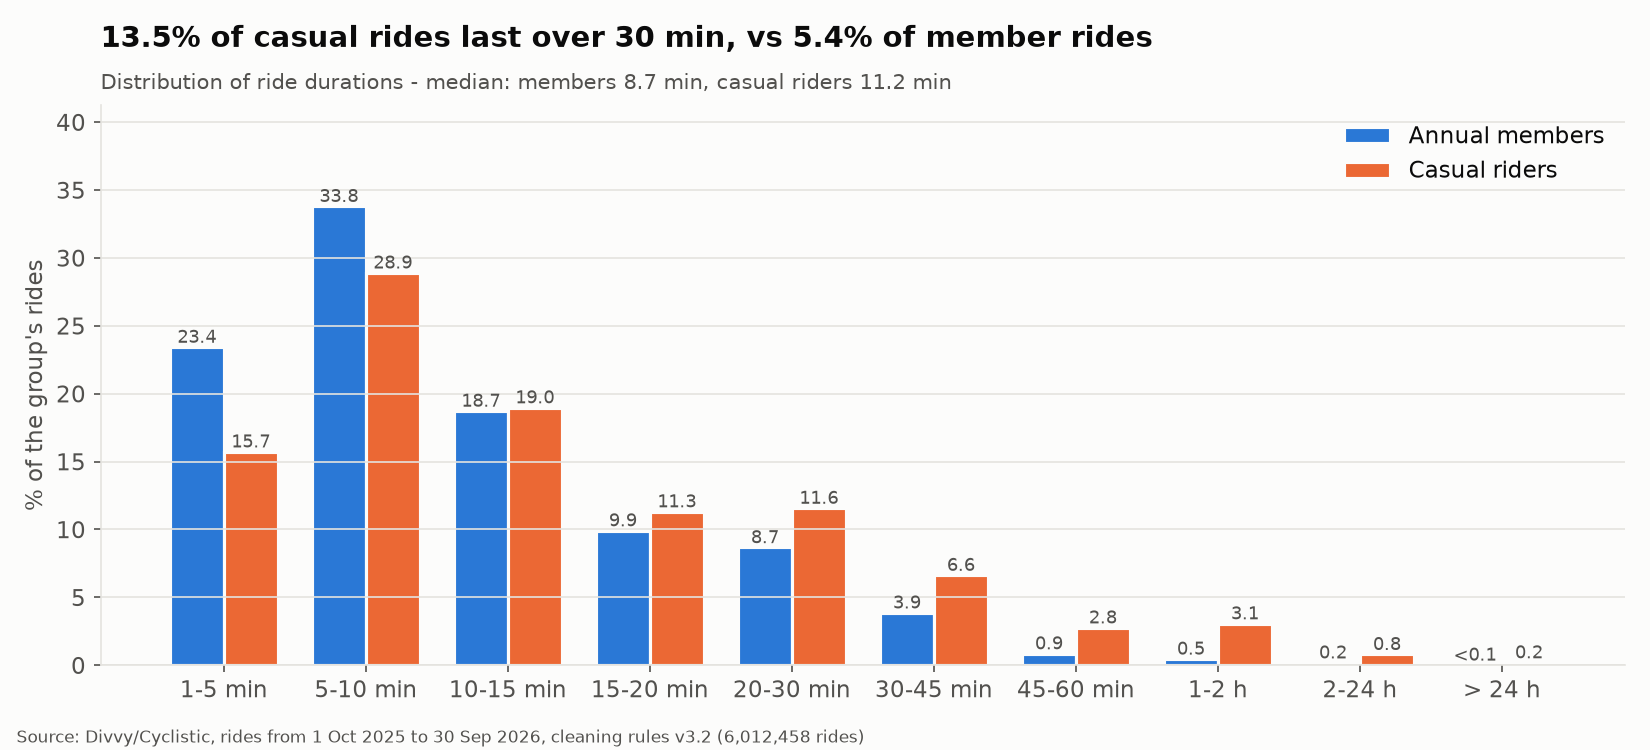
\includegraphics[width=0.94\linewidth]{f2_duration_distribution.png}
\caption{\textbf{Do both groups ride for as long?} No: rides of 1 to 10~min dominate among members (57.3\%), while casual riders are over-represented beyond 15~min; 13.5\% of their rides exceed 30~min, vs 5.4\%. \textit{(\file{f2\_duration\_distribution.png})}}
\label{fig:durations}
\end{figure}

\begin{figure}[H]
\centering
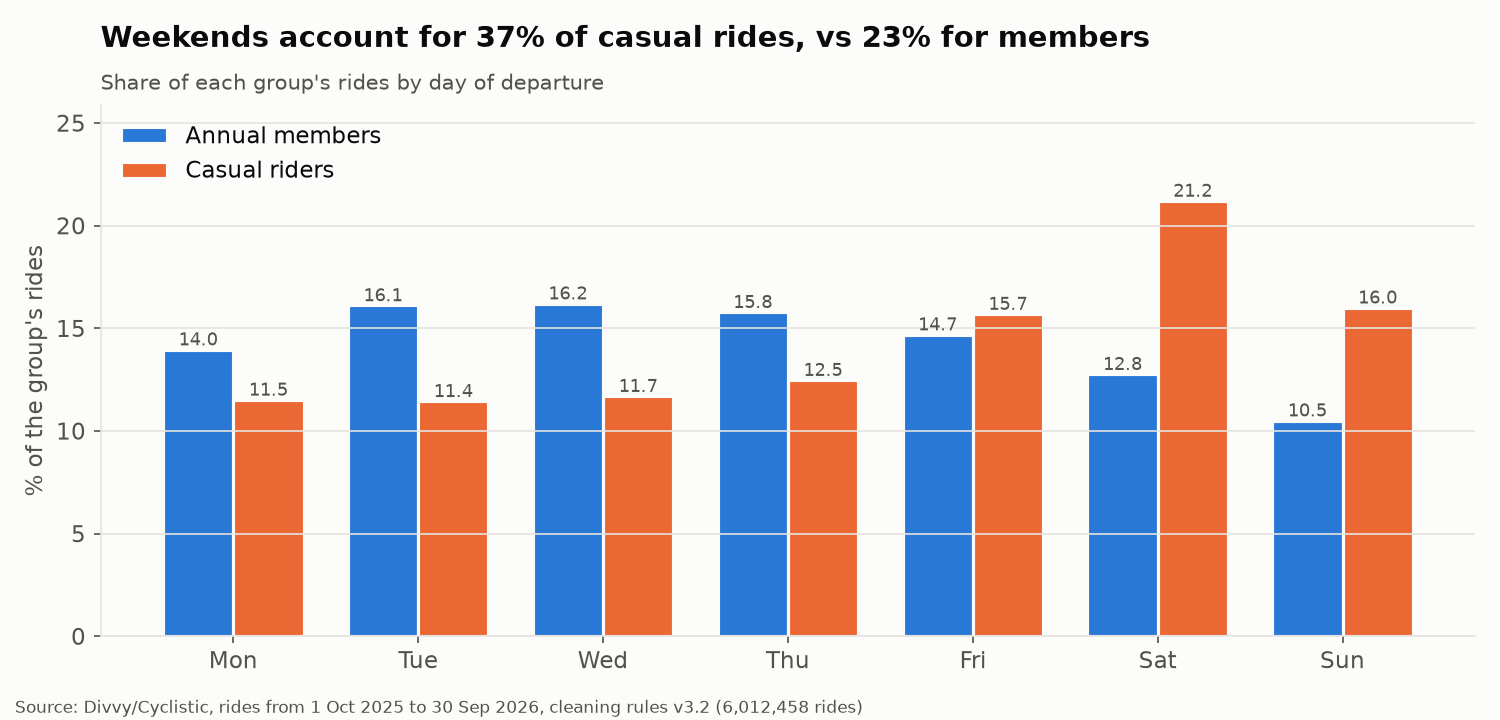
\includegraphics[width=0.94\linewidth]{f3_day_of_week.png}
\caption{\textbf{Do both groups ride on the same days?} Casual riders are over-represented at weekends (37.2\% of their rides vs 23.3\%), but most of their rides take place on weekdays. \textit{(\file{f3\_day\_of\_week.png})}}
\label{fig:days}
\end{figure}

\begin{figure}[H]
\centering
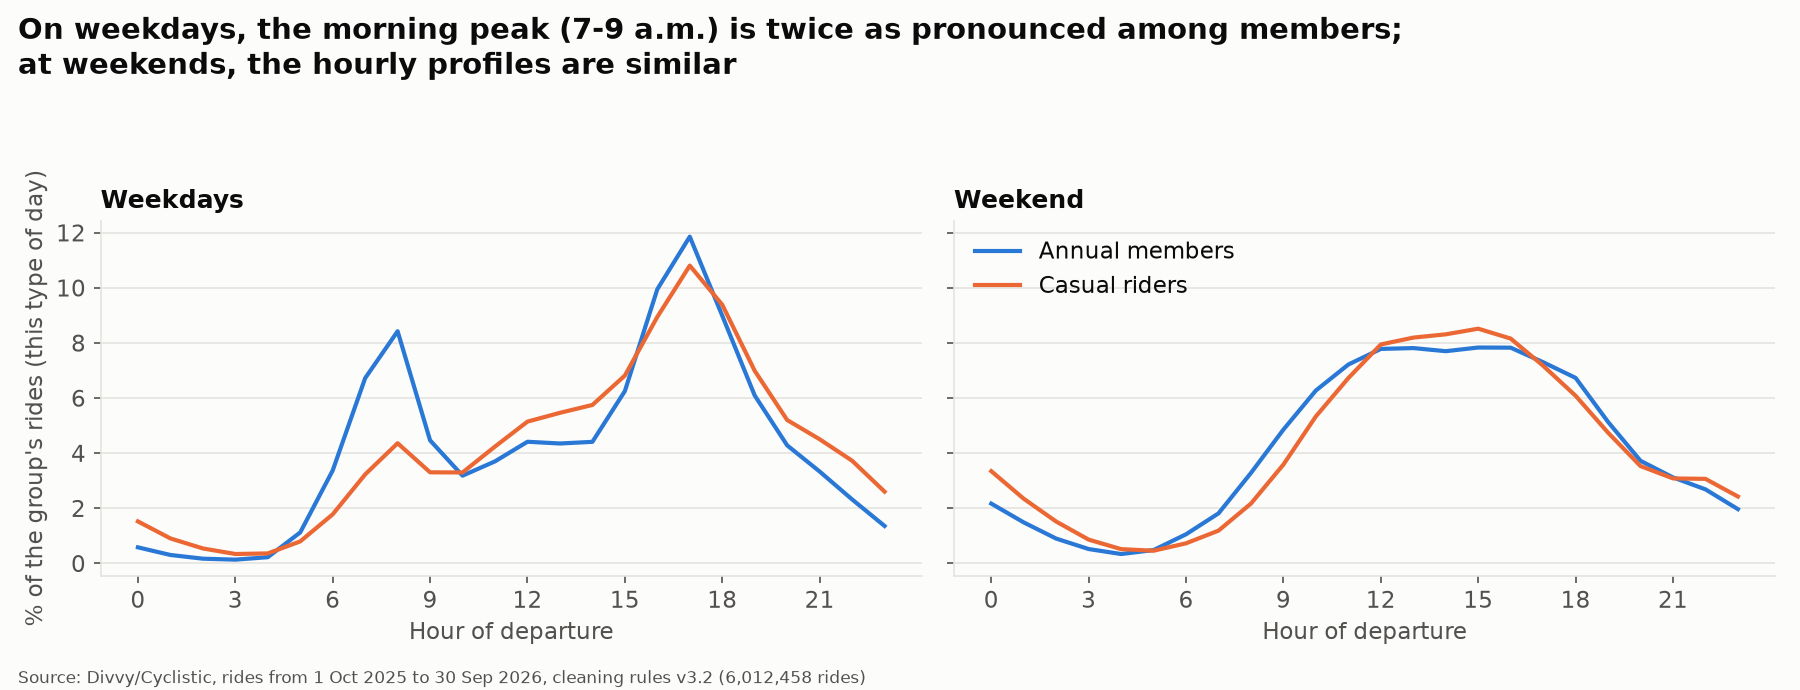
\includegraphics[width=0.98\linewidth]{f5_hourly_profile.png}
\caption{\textbf{At what time do they set off?} On weekdays, the morning peak (7--9 a.m.) is twice as pronounced among members; both groups peak at 5 p.m.; at weekends, the profiles are almost identical. \textit{(\file{f5\_hourly\_profile.png})}}
\label{fig:hours}
\end{figure}

\begin{figure}[H]
\centering
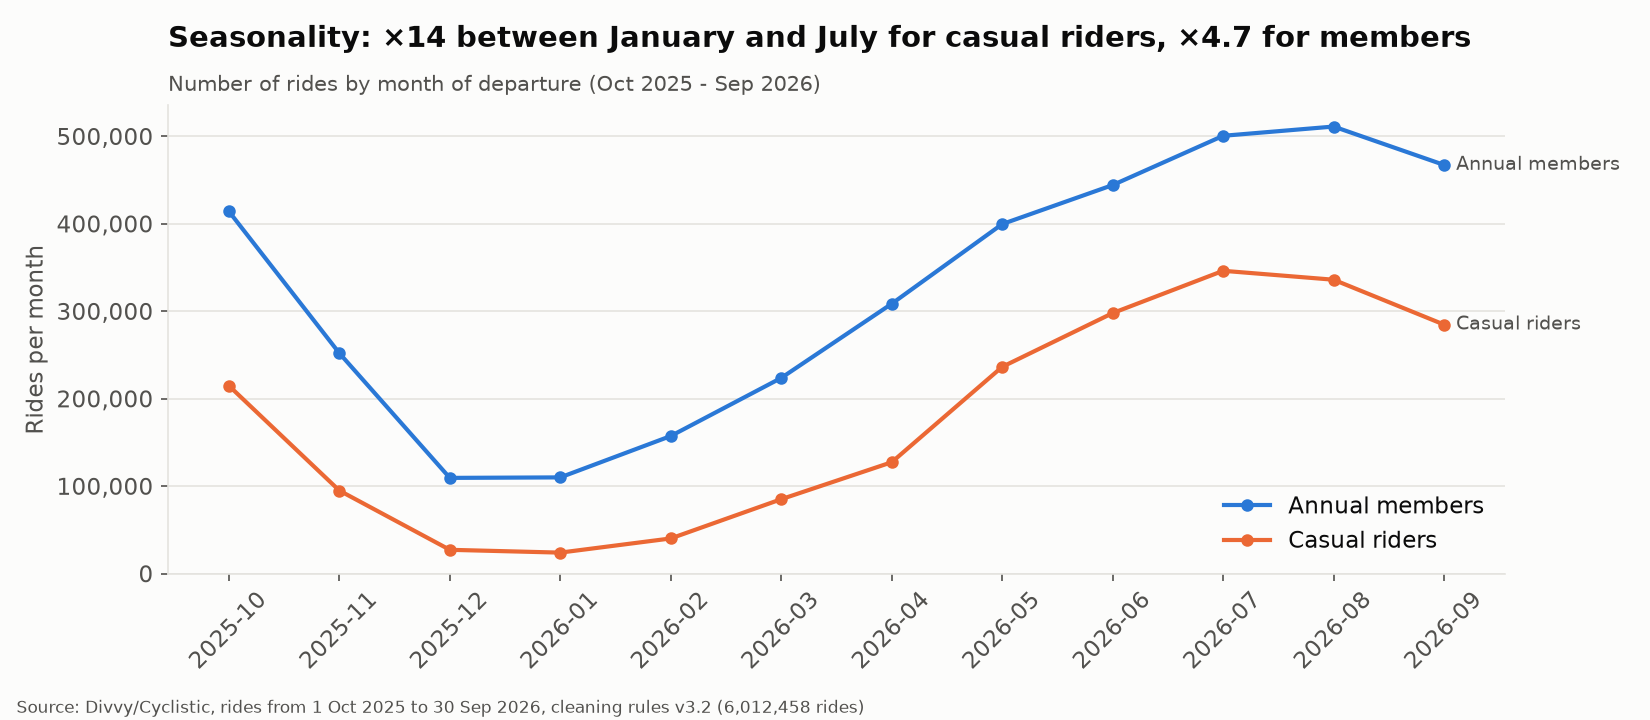
\includegraphics[width=0.94\linewidth]{f4_monthly_trend.png}
\caption{\textbf{Does usage vary with the season?} Same calendar, very different amplitude: ×14.4 between January and July for casual riders, ×4.7 between December and August for members. \textit{(\file{f4\_monthly\_trend.png})}}
\label{fig:months}
\end{figure}

\begin{figure}[H]
\centering
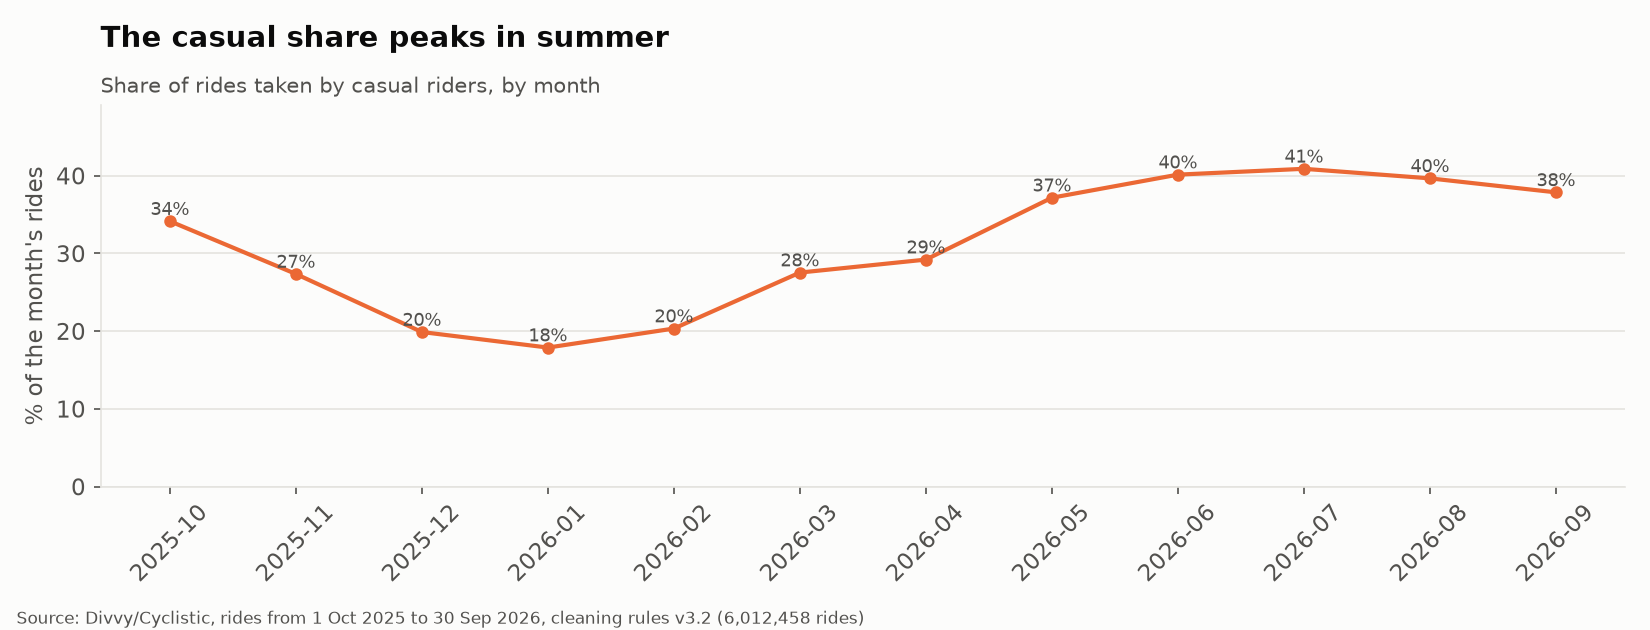
\includegraphics[width=0.94\linewidth]{f4b_casual_share_by_month.png}
\caption{\textbf{What share of activity do casual riders represent over the year?} From 17.9\% of rides in January to 40.9\% in July; more than 37\% from May to September. \textit{(\file{f4b\_casual\_share\_by\_month.png})}}
\label{fig:casualshare}
\end{figure}

\begin{figure}[H]
\centering
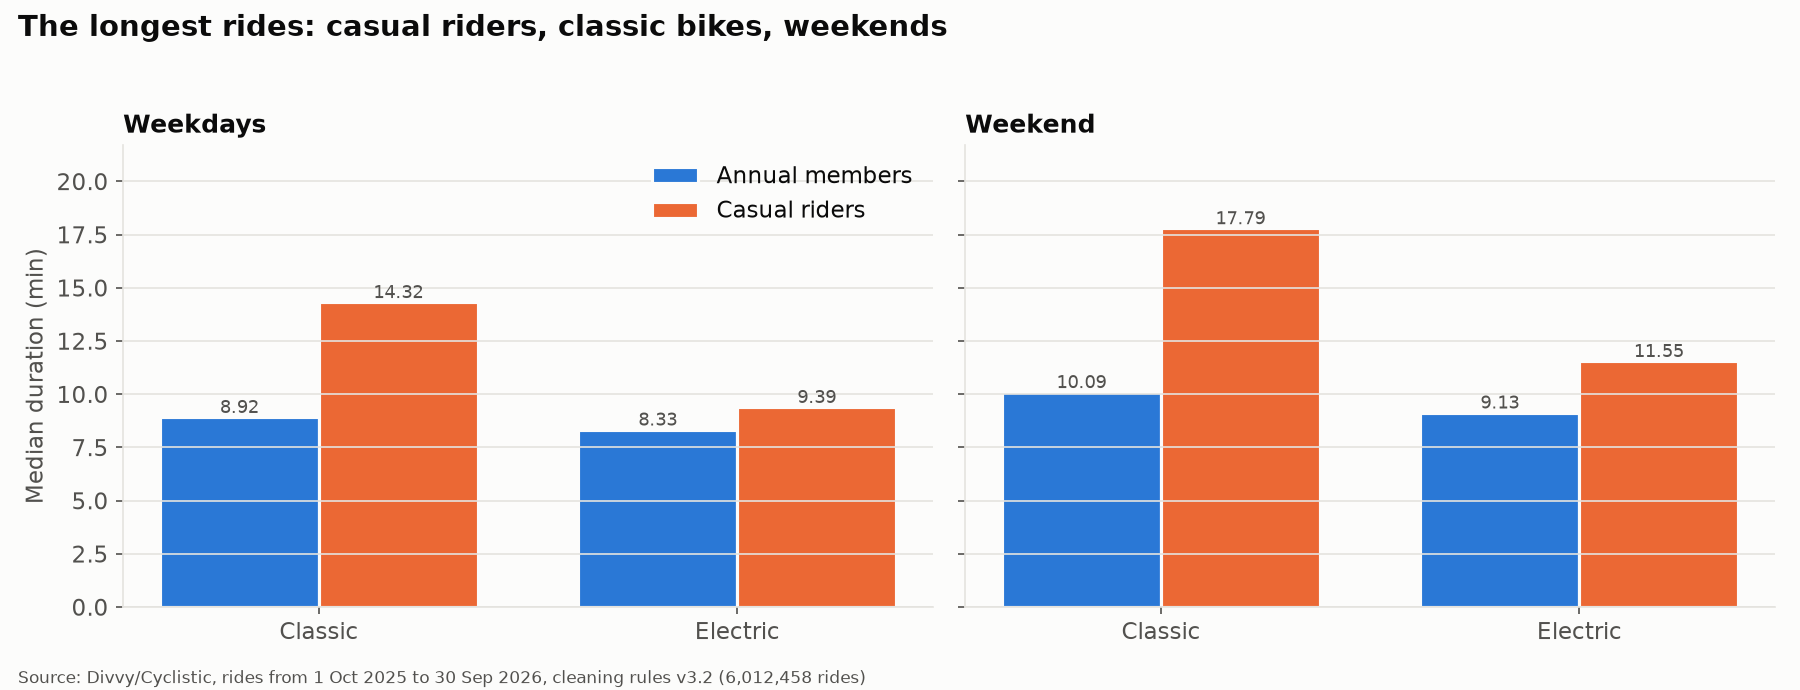
\includegraphics[width=0.98\linewidth]{f7_bike_type_by_day_type.png}
\caption{\textbf{Where is the duration gap largest?} On classic bikes at weekends (median 17.79 vs 10.09~min); on e-bikes on weekdays, the two groups are close (9.39 vs 8.33~min). \textit{(\file{f7\_bike\_type\_by\_day\_type.png})}}
\label{fig:bikes}
\end{figure}

\begin{figure}[H]
\centering
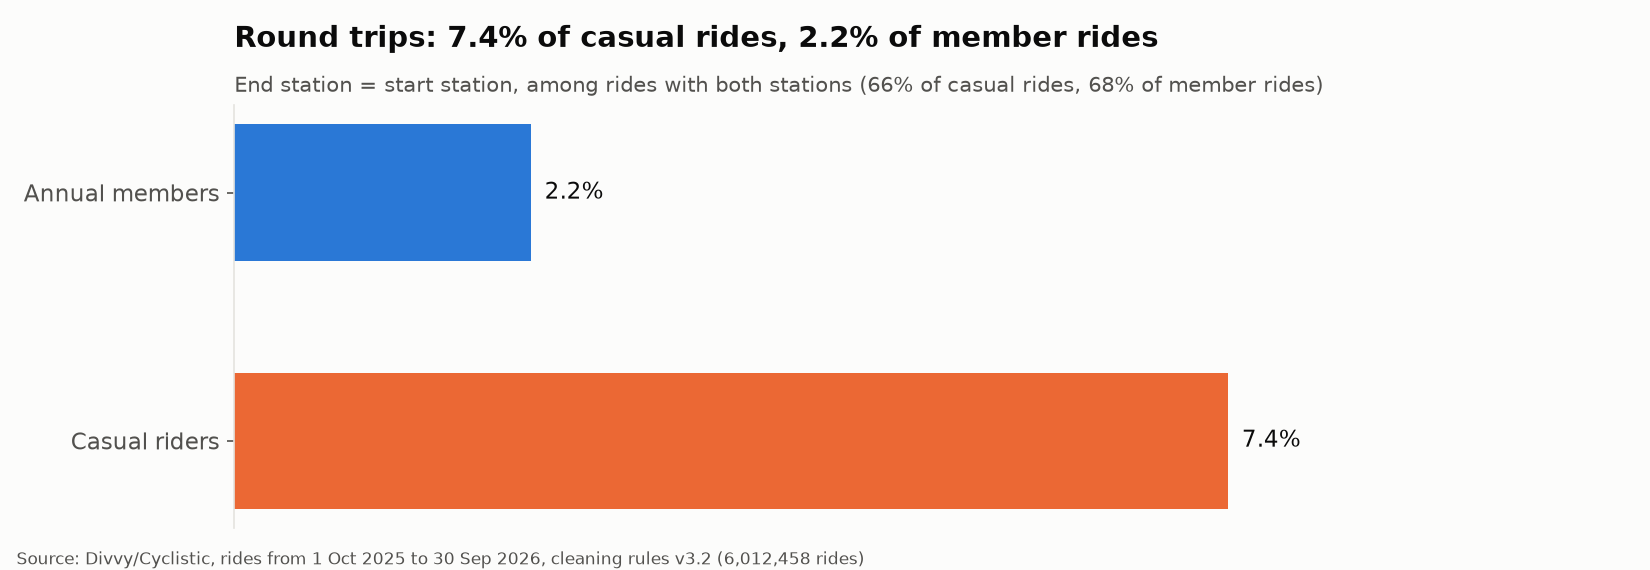
\includegraphics[width=0.86\linewidth]{f8_round_trips.png}
\caption{\textbf{Do rides return to their starting point?} 7.4\% of casual rides vs 2.2\% of member rides, among rides with both stations. \textit{(\file{f8\_round\_trips.png})}}
\label{fig:roundtrips}
\end{figure}

\section{Key insights}
\label{sec:insights}

\begin{enumerate}
  \item \textbf{Two distinct usage patterns.} \Mes{} Short, regular weekday rides for members; longer rides, more frequent at weekends, in the afternoon and in summer, for casual riders. \Int{} The first pattern is consistent with utilitarian trips, the second with leisure.
  \item \textbf{A measurable bridge.} \Mes{} 62.8\% of casual rides take place on weekdays; 23.1\% start on weekdays during peak hours (35.3\% for members). \Int{} Part of casual usage already resembles that of members.
  \item \textbf{The season concentrates the potential.} \Mes{} 71.0\% of casual rides take place from May to September; their share of all rides peaks at 40.9\% in July.
  \item \textbf{Duration mainly sets leisure rides apart.} \Mes{} The duration gap is largest for classic bikes at weekends and almost zero for e-bikes on weekdays.
  \item \textbf{Robust findings, unknown causes.} \Mes{} The differences hold in the sensitivity analyses. \Int{} The data reveal neither why a rider chooses a pass over a membership, nor how many people take these rides.
\end{enumerate}

\section{Three marketing recommendations}
\label{sec:recos}

Each recommendation starts from a measured finding \Mes{}; the proposed action is a hypothesis \Hyp{} whose effectiveness must be demonstrated through experimentation before any large-scale roll-out.

\begin{table}[H]
\caption{Overview of the recommendations}
\label{tab:recos}
\small
\begin{tabularx}{\linewidth}{c L{4.1cm} Y L{2.6cm}}
\toprule
\thead{\#} & \thead{Recommendation} & \thead{Main finding} & \thead{Evaluation} \\
\midrule
1 & Convert casual riders with utilitarian usage & 23.1\% of casual rides: weekdays, peak hours; shared peak at 5 p.m. & A/B test \\
2 & Leisure-oriented spring--summer campaign & 71.0\% of casual rides from May to September; 37.2\% at weekends & Test and control areas \\
3 & Digital communication on ride duration and e-bikes & 25.1\% of casual rides last at least 20~min; 74.1\% on e-bikes & A/B test between variants \\
\bottomrule
\end{tabularx}
\end{table}

% ---------------------------------------------------------------------------------
\newcommand{\recoline}[2]{\textbf{#1}\quad #2\par\smallskip}

\subsection{Recommendation 1 — Convert casual riders with utilitarian usage}
\recoline{Finding \Mes}{23.1\% of casual rides (487,667 rides) start on weekdays during peak hours, vs 35.3\% for members; the 5 p.m. peak is shared by both groups; on e-bikes on weekdays (47.5\% of casual rides), their median duration (9.39~min) is close to that of members (8.33~min).}
\recoline{Target audience}{Casual riders who ride regularly on weekdays during peak hours, to be identified in Cyclistic's customer accounts (the analyzed data set does not allow this).}
\recoline{Action \Hyp}{In-app and email message triggered after these rides, presenting the membership as the plan for everyday trips; a trial offer whose amount is still to be set by the finance team.}
\recoline{Timing}{Weekdays, from March to May, when activity picks up and before the summer peak.}
\recoline{Success metric}{60-day conversion rate of exposed accounts; in addition, the share of peak-hour rides taken by members (73.8\% today).}
\recoline{To validate}{The commuting motive is assumed; the effect of price is unknown.}

\subsection{Recommendation 2 — Leisure-oriented spring--summer campaign}
\recoline{Finding \Mes}{71.0\% of casual rides take place from May to September; their share reaches 40.9\% of rides in July; 37.2\% of their rides take place at weekends, including 21.2\% on Saturdays; round trips are 3.4 times more frequent than among members.}
\recoline{Target audience}{Leisure casual riders: weekends, warm season, long rides or round trips.}
\recoline{Action \Hyp}{Campaign on social media and in the app, presence at the busiest leisure stations; test a seasonal plan (a product and pricing decision, outside the scope of this analysis).}
\recoline{Timing}{From April to June, with highlights on Fridays and Saturdays.}
\recoline{Success metric}{New annual memberships in test areas compared with control areas.}
\recoline{To validate}{No weather or price data; a single year; leisure stations to be identified once station identifier consistency has been decided; occasional visitors may be hard to convert.}

\subsection{Recommendation 3 — Digital communication on ride duration and e-bikes}
\recoline{Finding \Mes}{25.1\% of casual rides last at least 20~min (14.1\% for members); on classic bikes at weekends, their median duration is 17.79~min vs 10.09~min; 74.1\% of their rides are on e-bikes.}
\recoline{Target audience}{Casual riders who take long rides or mainly use e-bikes.}
\recoline{Action \Hyp}{Message triggered after a long ride: cost of the pass used compared with the membership, calculated on the actual price list; member benefits on e-bikes, if the offer includes any. This also addresses Lily Moreno's question 3 on digital media.}
\recoline{Timing}{Right after the ride, during the active season.}
\recoline{Success metric}{Click-through rate and conversion rate by message variant.}
\recoline{To validate}{No price data: the savings for the rider must be checked with the finance team before any communication; exclude anomalous rides longer than 24~hours.}

\section{Evaluation framework for the recommendations}
\label{sec:measurement}

The primary metrics measure conversions and require Cyclistic's account data; the secondary metrics, which can be computed from the rides, provide context and \textbf{do not prove} on their own the effect of an action.

\begin{table}[!htbp]
\caption{Tracking metrics and baseline values}
\label{tab:kpi}
\small
\begin{tabularx}{\linewidth}{c Y L{2.6cm} L{3.0cm}}
\toprule
\thead{Rec.} & \thead{Metric} & \thead{Current baseline} & \thead{Data required} \\
\midrule
1 & \textbf{Primary:} 60-day conversion, exposed group vs control group & not available & accounts, memberships, A/B assignment \\
1 & Share of weekday peak-hour rides taken by members & 73.8\% & rides \\
2 & \textbf{Primary:} new memberships, test areas vs control areas & not available & memberships by area \\
2 & Casual share of rides in April, May, June & 29.2 / 37.2 / 40.1\% & rides \\
3 & \textbf{Primary:} clicks and conversions by message variant & not available & message logs, accounts \\
3 & Share of rides lasting at least 30~min, casual / members & 13.5 / 5.4\% & rides \\
\bottomrule
\end{tabularx}
\par\smallskip{\footnotesize\color{muted}Baselines computed from the rides of October 2025 to September 2026; source tables in \file{results/analysis/}: \file{a02\_durees\_tranches.csv}, \file{a04\_mois.csv} and \file{a05\_heure.csv}.}
\end{table}

\textbf{Evaluation protocol.}
\begin{itemize}
  \item \textbf{Systematic control group:} random assignment (A/B test) for recommendations 1 and 3; comparable control areas, using difference-in-differences, for recommendation 2.
  \item \textbf{Like-for-like periods:} seasonality (×14 for casual riders) makes any month-to-month comparison misleading.
  \item \textbf{Success criterion set in advance:} minimum conversion uplift deemed useful by management, sample size calculated before launch.
  \item \textbf{Same calculation rules:} baselines recomputed with the same scripts and the same cleaning rules (v3.2) to remain comparable.
\end{itemize}

\section{Limitations and next steps}
\label{sec:limitations}

\begin{minipage}[t]{0.485\linewidth}
\begin{keyboxfixed}[Limitations]\raggedright
\setlength{\parskip}{0pt}\begin{itemize}[leftmargin=1.1em, topsep=2pt, itemsep=3pt, parsep=0pt]
  \item Rides, not people: no customer count and no individual frequency.
  \item No prices, pass types, weather or demographic data.
  \item A single year observed.
  \item Provisional 60~s threshold (e-bikes only); conclusions unchanged in the sensitivity analysis.
  \item Source characteristics: March--April boundary, end of period, daylight saving time changes (474 rides not corrected in the fall).
\end{itemize}
\end{keyboxfixed}
\end{minipage}\hfill
\begin{minipage}[t]{0.485\linewidth}
\begin{keyboxfixed}[Further analysis]\raggedright
\setlength{\parskip}{0pt}\begin{itemize}[leftmargin=1.1em, topsep=2pt, itemsep=3pt, parsep=0pt]
  \item Station-level analysis (departures, arrivals, round trips), once station identifier consistency has been decided.
  \item Identification of ``utilitarian'' casual riders by station and by month.
  \item Combination with weather data to isolate the seasonal effect.
  \item Commercial data (passes, prices, conversions) to move from usage patterns to levers.
  \item Distances computed from coordinates, to complement duration.
\end{itemize}
\end{keyboxfixed}
\end{minipage}

\medskip
\textbf{Decisions still open.} Consistency criterion for station identifiers; rule for 41 rides linked to test or staff stations (kept); documentary correction of a check's reference value; access to account, price and pass data.

\section{Conclusion}
\label{sec:conclusion}

Across 6,012,458 rides from October 2025 to September 2026, annual members and casual riders use Cyclistic in two clearly different ways: short, regular weekday trips for the former; longer rides, at weekends and in the warm season, for the latter.
These differences are measured, consistent across tables and charts, and stable in the sensitivity analyses.

Yet a substantial share of casual rides already resembles member usage: this is the proposed priority target.
The three recommendations turn these findings into testable actions, each with a metric and a control group.
They remain hypotheses until they have been evaluated on Cyclistic's account and pricing data; the next step is to obtain these data and to launch recommendation~1 as an A/B test in the spring.

\appendix
\section{References}
\label{sec:refs}

\begin{enumerate}[label={[\arabic*]}, leftmargin=2em]
  \item Google, \emph{Case Study 1: How does a bike-share navigate speedy success?}, Google Data Analytics Professional Certificate (document provided to learners, accessed October 2026).
  \item Divvy, historical trip data: \url{https://divvy-tripdata.s3.amazonaws.com/index.html} (12 monthly files, October 2025 to September 2026, downloaded on 11~October 2026).
  \item Divvy, \emph{Data License Agreement} (Lyft Bikes and Scooters, LLC; data owned by the City of Chicago): \url{https://www.divvybikes.com/data-license-agreement}, accessed October 2026. The case study refers to the data as made available by Motivate International Inc.
  \item Divvy, \emph{System Data} (data processing, including the removal of rides shorter than 60~seconds): \url{https://divvybikes.com/system-data}, accessed on 11~October 2026.
  \item P. Wagler, J. MacFarlane, \emph{Eisvogel}, LaTeX template for pandoc, BSD 3-Clause license: \url{https://github.com/Wandmalfarbe/pandoc-latex-template} (basis of this report's layout).
\end{enumerate}

\section{Reproducibility}
\label{sec:repro}

\begin{table}[H]
\caption{Processing pipeline and associated files}
\label{tab:repro}
\small
\begin{tabularx}{\linewidth}{L{3.4cm} Y}
\toprule
\thead{Step} & \thead{Files (project repository)} \\
\midrule
Cleaning rules & \file{docs/plan\_nettoyage\_v3.2.md}, \file{config/regles\_nettoyage\_v3.2.json} \\
Cleaning and checks & \file{scripts/run\_clean.py}, \file{sql/02\_clean.sql}, \file{sql/03\_qa\_clean.sql} \\
Quality results & \file{docs/methodology.md}, \file{results/quality/} \\
Analysis aggregations & \file{sql/10\_analyse.sql}, \file{scripts/run\_analyse.py} $\rightarrow$ \file{results/analysis/} \\
Charts & \file{scripts/figures\_analyse.py} $\rightarrow$ \file{visualizations/} \\
Sensitivity analyses & \file{sql/04\_sensitivity.sql}, \file{scripts/run\_sensitivity.py} $\rightarrow$ \file{results/quality/} \\
This report & \file{scripts/generate\_latex\_tables.py}, \file{scripts/build\_latex\_report.py}, \file{reports/latex/} \\
\bottomrule
\end{tabularx}
\end{table}

The numerical tables in this report are generated from the analysis CSV files; the numbers quoted in the text are checked automatically by \file{scripts/build\_latex\_report.py} before each build. Build instructions are given in \file{reports/latex/README.md}.

\end{document}
